\subsection{Background}


The city of Madison presents a significant opportunity for the implementation of electric vehicle (EV) charging infrastructure. There are a plethora of available parking lots in the city, each of which has the potential to serve a specific region and meet the demands of local parking needs. In particular, the downtown and campus areas of Madison exhibit a higher density of parking lots, reflective of the increased demand for parking in these areas. In light of this, it is assumed that all EV charging stations will be situated within existing parking lots, as EVs typically utilize their parking time for charging. Furthermore, indoor parking lots provide an optimal environment for EV charging, as their construction design can facilitate the maintenance of desirable temperature and voltage levels, which are crucial for effective battery charging.

To simplify the model, the city of Madison has been divided into sixteen equally-sized areas, with two parking lots assumed to cover each area. This model can be easily adapted to account for additional parking lots and different area divisions, providing a flexible framework for the implementation of EV charging infrastructure in Madison.
\begin{figure}[t]
    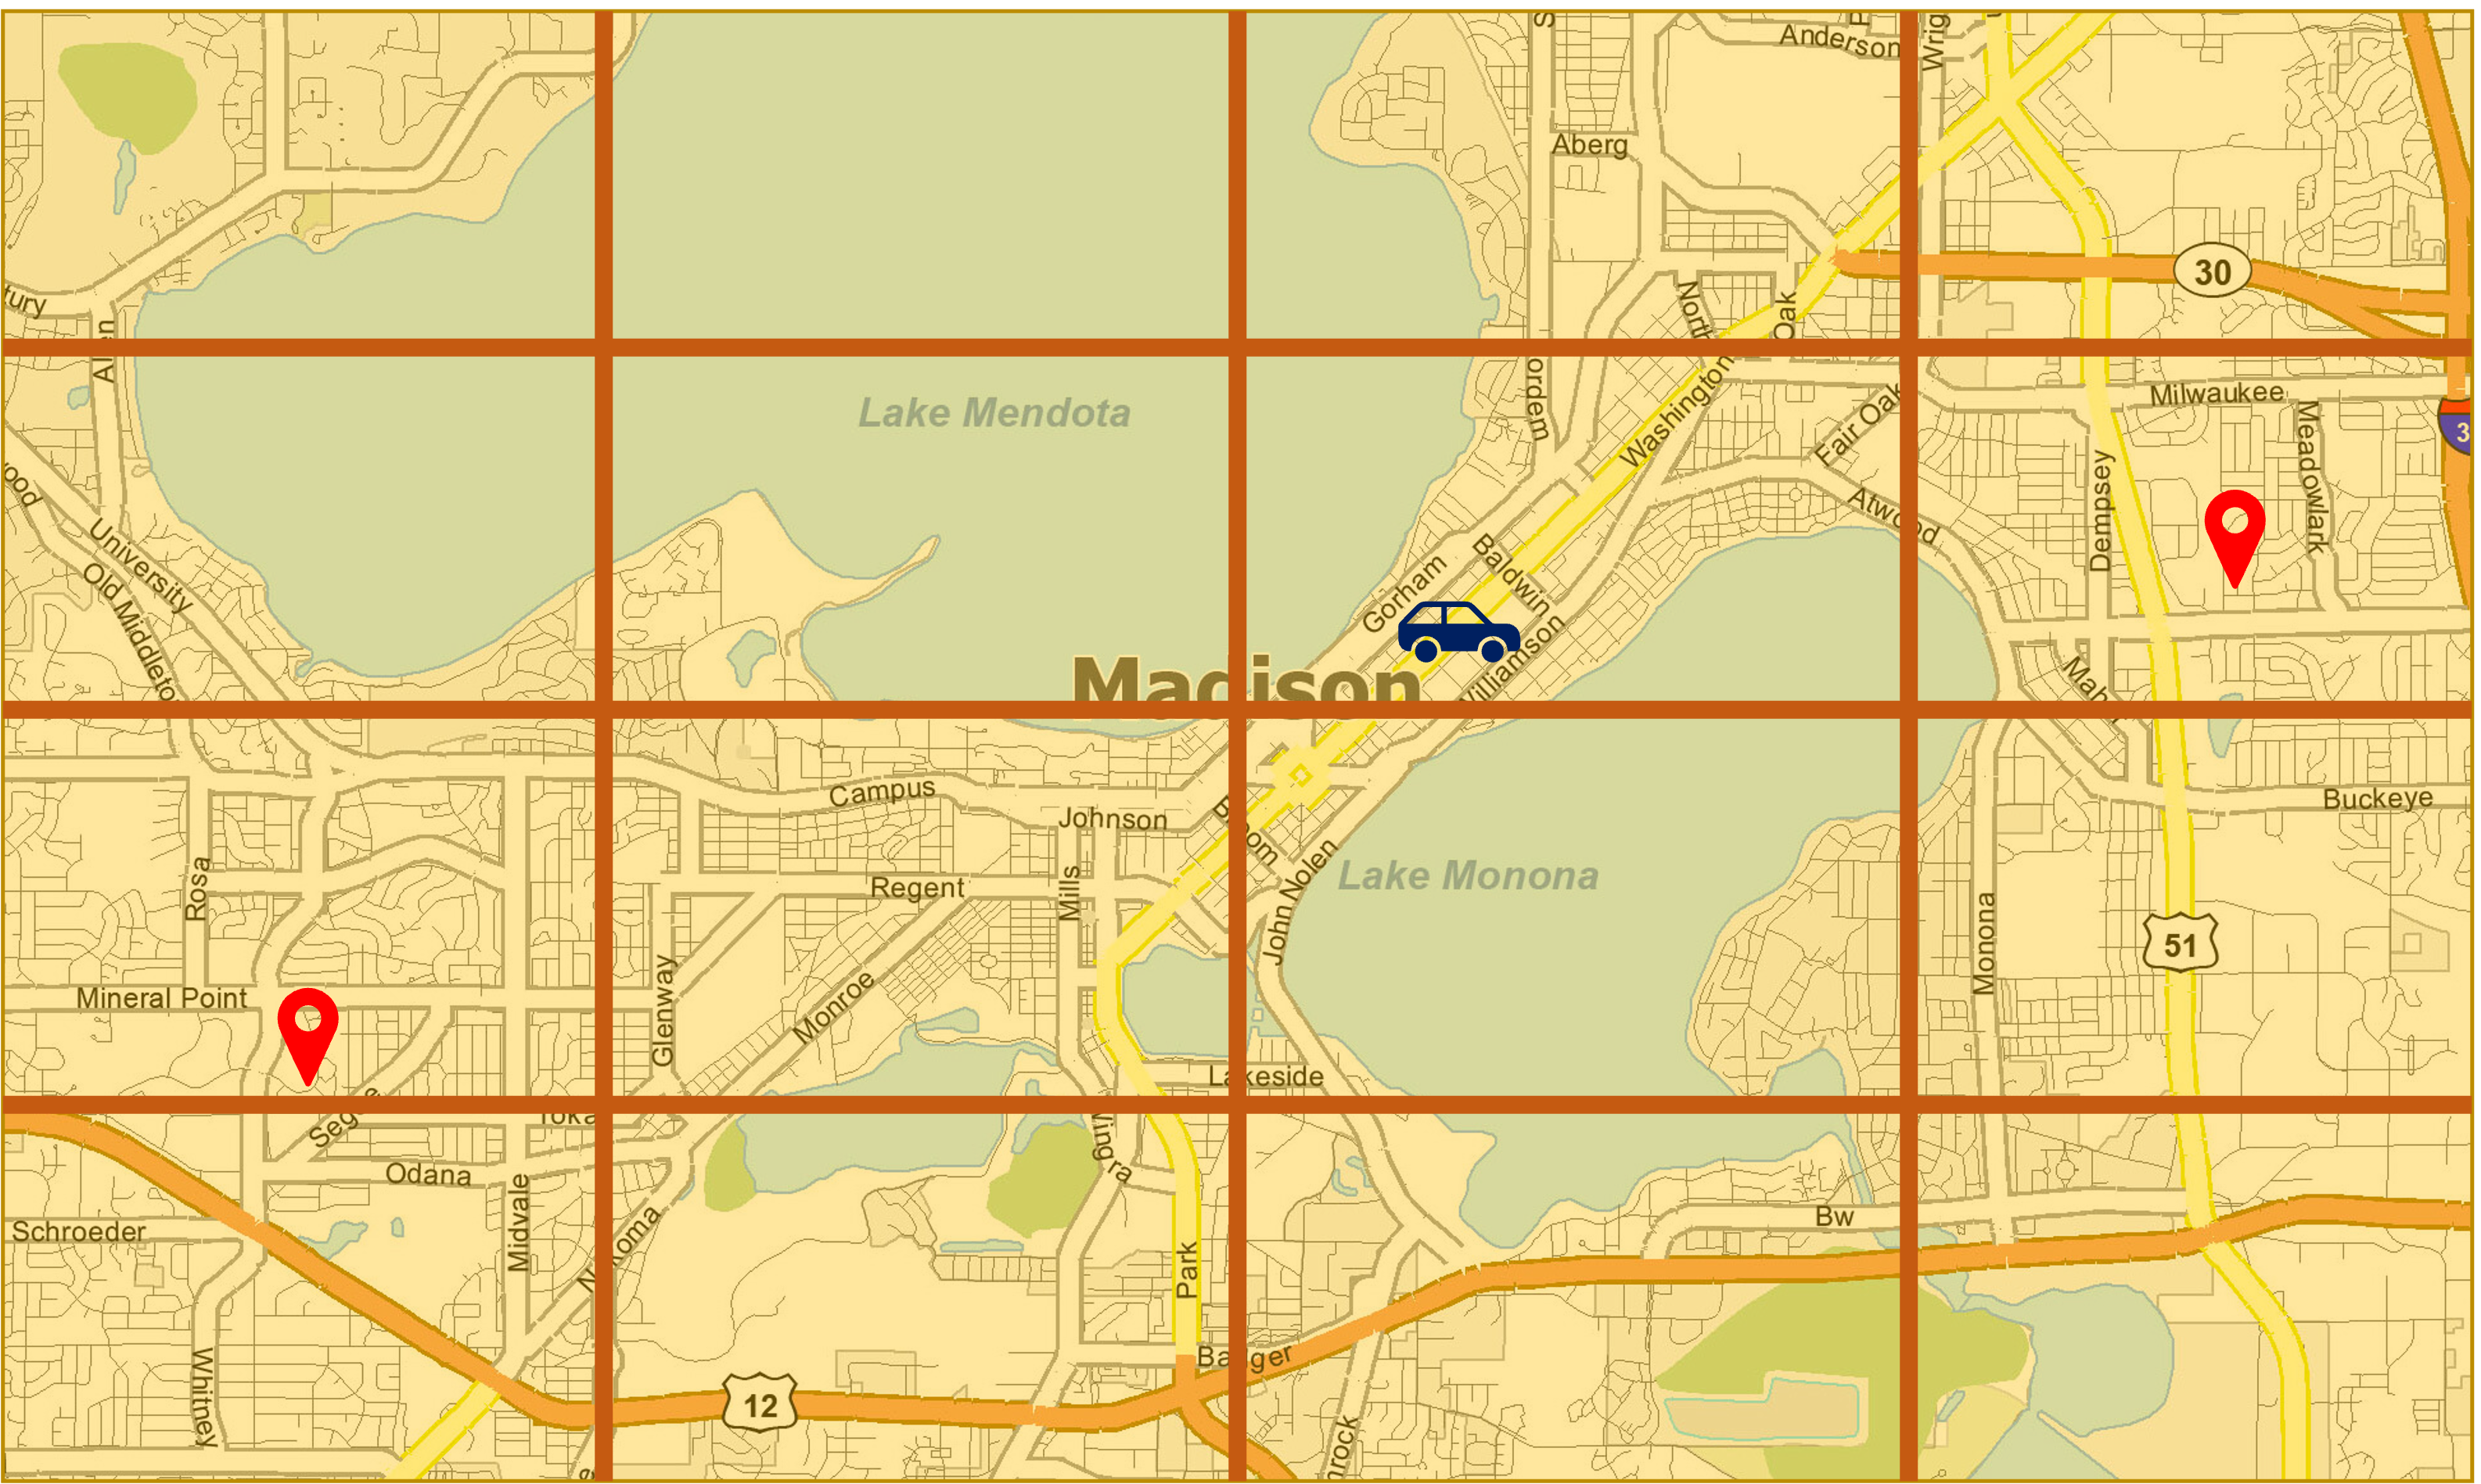
\includegraphics[width = 0.8\textwidth]{figure/madison.png}
    \centering
    \caption{The city division and parking lots assumption}
    \label{fig:madison}
\end{figure}


\subsection{Model Overview}
In order to accurately simulate the scenario of EV charging infrastructure implementation in Madison, a comprehensive model was developed that is divided into three key components: Data Generation, Drivers' Choice, and Parking Simulation. The flowchart~\ref{fig:flowchart} provided illustrates the structure of the model and the inter-dependencies between the various components.

Given the paucity of available data, the Data Generation component of the model is crucial in generating synthetic data to be used in the subsequent stages of the model. As such, the validity of the results obtained is contingent upon the quality of the data generated. However, when real-world data becomes available, it can be easily integrated into the model by modifying the Data Generation component, thereby enabling the generation of results that are reflective of reality.

\begin{figure}[t]
    \includegraphics[width = 0.9\textwidth] {figure/flowchart.png}
    \centering
    \caption{The overall structure of the model}
    \label{fig:flowchart}
\end{figure}


\subsection{Model Details}
\subsubsection{Data Generation}
Due to the lack of available data, the Data Generation component of the model is crucial in generating synthetic data to be used in the subsequent stages of the model. As such, the validity of the results obtained is contingent upon the quality of the data generated. However, when real-world data becomes available, it can be easily integrated into the model by modifying the Data Generation component, thereby enabling the generation of results that are reflective of reality.

\textbf{Scenario}: In our model, we analyze parking and charging occurrences for electric vehicles (EVs) within two distinct scenarios: normal days and Game days. For normal days, we posit an even distribution of traffic across all regions. However, during Game days, due to the high demand for parking in close proximity to the stadium, we predict that certain parking lots will experience heavy traffic influx during specific time periods.

For simplicity, we adopt a uniform distribution of incoming traffic flow during normal days. This assumption implies that vehicles arrive at the parking lots at consistent intervals, reflecting an evenly distributed arrival pattern. Conversely, for Game days, we model a more concentrated traffic flow, with 80\% of incoming traffic arriving during 10\% of the day to mimic the intense short-term demand typically observed during such events.


\textbf{Price}: Pricing is another crucial factor in our model, which is considered to significantly influence a driver's choice of parking location. We allow the parking price to either be a fixed value or selected dynamically within a specific range. In the context of Game days, we introduce a \textit{Game-day multiplier} to adjust the prices dynamically, allowing us to assess the impact of such price modifications on parking and charging behavior.

\textbf{Spots}: Spots refer to the available chargers in certain parking lots, and we also considered this as one of the factors that will influence the driver's decision. Given a specific budget, we assume a limited total number of available chargers to be installed citywide. In most of our experimentations, we set this total to be 20, symbolizing a resource-constrained scenario.

\textbf{Distance(Pref)}: Distance refers to the proximity of the parking lot to the driver's intended destination. It is generally understood that drivers prefer to park as close to their destination as possible. Consequently, the `distance preference' can be interpreted as the relative desirability of a parking lot for each driver: the shorter the distance to the destination, the higher the preference for the parking lot. We generate these values from a uniform distribution within a specific range for our simulations.

\subsubsection{Choice Model}

In analyzing the behavior of electric vehicle (EV) drivers when choosing a parking lot, we consider their choice as a utility-based decision. To capture the decision-making process accurately, we propose a model based on the renowned Cobb-Douglas utility function. This function, when supplied with input variables related to parking price, available charging spots, and distance to the destination, yields a utility value for each parking lot from the perspective of a given driver. 

Drivers then make their choices based on these calculated utility values. A higher utility value increases the likelihood of a particular parking lot being selected by a driver. The probabilistic element in our model serves to account for the unexpected and non-linear decisions that real-world drivers may make. 

To explicate further, the utility function for the i-th driver (represented by \(d_i\)) for a specific parking lot (represented by \(l\)) is denoted as:

\[
\mu_{d_i}(l) = P_l^{\alpha} S_l^{\beta} D_l^{\gamma}
\]

In this equation, \(P_l\) denotes price at parking lot $l$, \(S_l\) represents the available charging spots, and \(D_l\) stands for distance to the desired destination. The parameters \(\alpha\), \(\beta\), and \(\gamma\) are tuned for the simulation, dictating the weight of each factor in the utility calculation. Here we ignored the differences between individual drivers and selected uniform parameters for all drivers.

Subsequently, the decision function is defined as:

\[
\mathbb{P}_{d_i}(l) = Bin(1, \mu_{d_i}(l))
\]

The decision function essentially transforms the computed utility values into binary decisions, representing the selection or rejection of a parking lot.

By synthesizing the present location of each driver and their choices derived from the model, we can simulate the incoming flow to each parking lot, thus generating the \emph{Inflow Data}. This data provides valuable insights into the parking behavior of EV drivers under various circumstances and allows for a comprehensive analysis of parking lot utility in different scenarios.

\subsubsection{Parking Simulation}
The parking simulation can be broken down into several sequential phases: the entry process, the charging process, and the queueing process.

\paragraph{Entry Process}
Upon arriving at a given parking lot, a driver may encounter one of two scenarios: the parking lot currently has an available spot, or the parking lot is fully occupied necessitating a waiting queue.

Should an available spot be present, the driver proceeds to enter the lot and initiates the charging process. However, in the absence of an open spot, the driver is required to join the queue.

\paragraph{Charging Process}
Upon successful entry into the parking lot, the driver commences the charging process immediately. In this model, the time taken to locate a specific spot within the lot is disregarded, as it is not a primary concern within the scope of this model.

The duration of the charging process hinges on the current battery level of the vehicle and thus varies across drivers. To emulate this variability, a uniform distribution is employed to determine the requisite charging time for each driver.

\paragraph{Queueing Process}
If a driver fails to secure a spot in the parking lot and consequently joins the queue, they must follow the ensuing procedure.

The driver is obligated to wait for a minimum of one time unit. Their willingness to remain in the queue is quantified by the \emph{stay probability}. After each time unit, the stay probability reduces by a certain amount. If the stay probability falls below a predefined threshold, the driver abandons the queue and does not return. These drivers are counted as `rejected' drivers. 

At each time unit, the driver attempts to enter the parking lot, taking advantage of spots that may have become available due to other drivers completing their charging. The entry system operates on a first-come, first-served basis, thereby granting priority to drivers who joined the queue earlier and have not yet left.

Let the threshold be denoted by $p$ and the decrement amount by $\delta_p$. The queueing process can be succinctly represented using the following algorithm:

\begin{algorithm}
\caption{Driver Queueing Procedure}
\label{alg:entry}
\begin{algorithmic}[1]
\If{$P_{stay} > p$}
\If{$Spot > 0$}
\State Enter System
\State Remove Driver from Queue
\Else
\State $P_{stay} \gets P_{stay} - \delta_p$
\EndIf
\EndIf
\end{algorithmic}
\end{algorithm}

\subsection{Evaluation Model}
Our evaluation model takes into account perspectives from both drivers and infrastructure designers. From the driver's perspective, primary considerations include the successful service rate, preference satisfaction, and the cost of charging. Conversely, from the designer's viewpoint, the primary concern lies with the utilization rate of the chargers.

In greater detail, the driver-centric considerations are as follows:
\begin{enumerate}
    \item The successful service rate, defined as the proportion of drivers who successfully charge their cars relative to the total number of drivers. This metric is essential as drivers are primarily concerned with their ability to charge their vehicles rather than merely queueing and potentially being 'rejected' in the end.

    \item Preference satisfaction, quantified as the proportion of drivers content with their chosen parking lot relative to the total number of drivers. Given that drivers naturally desire to park as close as possible to their final destination, this factor is deemed crucial.

    \item The charging cost, which varies across parking lots. Typically, drivers prefer to pay less for identical services unless distance preferences hold greater appeal. The influence of pricing strategies in mitigating congestion at specific parking lots during Game Day scenarios forms a key discussion point in subsequent sections.
\end{enumerate}

To balance the focus between the driver and designer perspectives, we employ a satisfaction adjustment coefficient, denoted by $\theta$. The efficiency rate of the chargers also plays a pivotal role in striking a balance between these two considerations.

When the charger efficiency rate exceed a specified threshold, such as 75\%, driver satisfaction is prioritized. By adeptly balancing the preferences of drivers and infrastructure designers, our model is positioned to offer valuable insights for the evolution of EV charging infrastructure.

\subsection{Model Validation}
Model validation is essential to ensure the reasonability and consistency of our model's functionality. Given the inclusion of random factors in our model, we need to conduct simulations both with and without these factors to observe if the outcomes align with expectations.

\subsubsection{Baseline Test}
The simplest test involves eliminating all random elements and maintaining constant parameters across the board. In such a case, we expect a uniform distribution of results across all parking lots. We implement a policy that biases driver preference towards a specific parking lot over the others. The experiment operates under settings of 2 parking lots, 20 chargers, 70 drivers, 40 observed time units, and a charging time of 30 time units. The resulting data is demonstrated in Figure \ref{fig:baseline}.

\begin{figure}[htbp]
    \centering
    \includegraphics[width=\textwidth]{figure/baseline.png}
    \caption{Baseline Test}
    \label{fig:baseline}
\end{figure}

To understand the figure, it is bifurcated into two primary sections. The upper half outlines the specifics of the simulation, with the x-axis representing the time unit. The histogram depicts the occupancy of chargers at each specific time, the number of drivers in the queue, the count of vehicles that successfully enter the parking lot, and the number of drivers who exit the queue due to excessive waiting times. The last row indicates the incoming flow for the experiment.

The lower half showcases statistical attributes of the experiment, where the x-axis represents the settings (e.g., $[3,17]$ implies 3 chargers in the first parking lot and 17 chargers in the second). The green line signifies system efficiency, representing the occupancy rate of chargers over the entire observation period. The red line indicates the cumulative satisfaction score for each configuration, while the purple line outlines the overall target value computed by a weighted sum of efficiency and preference satisfaction. The last row compares the ratio of choice alteration with the ratio of charger modification. The yellow-green line exhibits the number of chargers relocated from one parking lot to another, and the olive line indicates the number of drivers who switch their parking lot choice in response to charger relocation.

The outcomes of this baseline test are sensible since we nullify all randomness and manually direct drivers to select the second parking lot. All drivers flood towards a single parking lot, and the efficiency rate is high when we allocate more chargers to one parking lot. This is because new cars continuously arrive for charging, reducing the likelihood of chargers remaining idle. The symmetry of the green and red lines is logical since it demonstrates consistent outcomes when the order of charger assignment is reversed. The red line remains constant because we eliminate the leaving mechanism. Thus, all drivers persist in waiting for service until the observation concludes, rendering the satisfaction score constant as they all select the same parking lot.

